% 3
%\chapter{線形無順序木パターンの質問学習}
\section{線形無順序木パターンの質問学習}

%2023年6月29日木曜日から7月1日土曜日まで沖縄科学技術大学院大学カンファレンス・センターにて行われた第143回数理モデル化と問題解決(MPS)と,2024年9月4日水曜日から9月6日金曜日まで広島工業大学五日市キャンパスにて行われた第23回情報科学技術フォーラム(FIT2024)で口頭発表を行った内容である.

% 3.1
\subsection{無順序木パターン言語の計算問題}
本章では,線形無順序木パターンの計算問題の時間計算量について述べる.
無順序項木パターン$t\in{\cal UTTP}_{\Sigma,\Lambda,X}$と無順序木$T=(V_T,E_T)$が与えられたとき,$T\in L(t)$か否かを決定する問題を次のように定義する.

\medskip
\noindent
\textbf{無順序項木パターン照合問題}(${\cal UTTP}$-${\cal MP}$)\\
\textbf{入力}: 無順序項木パターン$t\in {\cal UTTP}$と無順序木$T\in {\cal UT}$.\\
\textbf{問題}: $t$は$T$にマッチするか?
\medskip

無順序項木パターン照合問題は,$t$が線形無順序項木パターンであったとしても,次元4以上の変数が存在すればNP完全である\cite{shoudai-ieice2018}.
一方,全ての変数の次元が2であれば,無順序項木パターン$t\in {\cal UTTP}$と無順序木$T\in {\cal UT}$に対する無順序項木パターン照合問題は,$n$を$t$の頂点数,$N$を$T$の頂点数とするとき,$O(nN^{1.5})$時間で計算可能である\cite{shoudai-ieice2018}.従って,以下に示す線形無順序木パターン$t\in{\cal LUTP}_{\Sigma,\Lambda,X}$に対する無順序項木パターン照合問題は入力サイズの多項式時間で計算可能である.

\medskip
\noindent
\textbf{線形無順序木パターン照合問題}(${\cal LUTP}$-${\cal MP}$)\\
\textbf{入力}: 線形無順序木パターン$t\in {\cal LUTP}$と無順序木$T\in {\cal UT}$.\\
\textbf{問題}: $t$は$T$にマッチするか?
\medskip

次に,無順序項木パターン$t\in {\cal UTTP}$に対する無矛盾性問題を次のように定義する.

\medskip
\noindent
\textbf{無順序項木パターンに対する無矛盾性問題}(${\cal UTTP}$-${\cal CP}$)\\
\textbf{入力}: 無順序木の有限集合$S_+\subseteq {\cal UT}_{\Sigma,\Lambda}$と$S_-\subseteq {\cal UT}_{\Sigma,\Lambda}$,ただし$S_+\cap S_-=\emptyset$.\\
\textbf{問題}: $S_+\subseteq L(t)$かつ$S_-\cap L(t)=\emptyset$を満たす無順序項木パターン$t\in {\cal UTTP}_{\Sigma,\Lambda,X}$は存在するか?
\medskip

上記問題と同様に,無順序項木パターンを線形無順序項木パターン$t\in {\cal LUTTP}$に限定した\textbf{線形無順序項木パターンに対する無矛盾性問題}(${\cal LUTTP}$-${\cal CP}$)を次のように定める.

\medskip
\noindent
\textbf{線形無順序項木パターンに対する無矛盾性問題}(${\cal LUTTP}$-${\cal CP}$)\\
\textbf{入力}: 無順序木の有限集合$S_+\subseteq {\cal UT}_{\Sigma,\Lambda}$と$S_-\subseteq {\cal UT}_{\Sigma,\Lambda}$,ただし$S_+\cap S_-=\emptyset$.\\
\textbf{問題}: $S_+\subseteq L(t)$かつ$S_-\cap L(t)=\emptyset$を満たす線形無順序項木パターン$t\in {\cal LUTTP}_{\Sigma,\Lambda,X}$は存在するか?
\medskip

Miyanoら\cite{miyano-ngc2000}は正則パターンに対して定義された無矛盾性問題がNP完全であることを示した.次章で,${\cal LUTP}$-${\cal CP}$がNP完全であることを証明する.

% 3.2
\subsection{線形無順序木パターンに対する無矛盾性問題のNP完全性}
無順序木パターンは葉を子ポートとする次元2の変数しか現れない線形無順序項木パターンである.本章では,無順序木パターンの機械学習,特に二値分類問題に密接に関連する決定問題${\cal LUTP}$-${\cal CP}$がNP完全であることを証明する.

\medskip
\noindent
\textbf{線形無順序木パターンに対する無矛盾性問題}(${\cal LUTP}$-${\cal CP}$)\\
\textbf{入力}: 無順序木の有限集合$S_+\subseteq {\cal UT}_{\Sigma,\Lambda}$と$S_-\subseteq {\cal UT}_{\Sigma,\Lambda}$,ただし$S_+\cap S_-=\emptyset$.\\
\textbf{問題}: $S_+\subseteq L(t)$かつ$S_-\cap L(t)=\emptyset$を満たす無順序木パターン$t\in {\cal LUTP}_{\Sigma,\Lambda,X}$は存在するか?

以下では,$S_+$に属す無順序木を正例,$S_-$に属す無順序木を負例と呼ぶ.

% 定理1
\begin{theorem}
線形無順序木パターンに対する無矛盾性問題${\cal LUTP}$-${\cal CP}$はNP完全である.
\end{theorem}

\begin{proof}
線形無順序木パターンに対する無矛盾性問題がクラスNPに属すことは自明である.
NP完全であることが知られている充足可能性問題(3-SAT)から${\cal LUTP}$-${\cal CP}$への多項式時間帰着を示す.
$x_{1},\ldots,x_{n}$を$n$ $(n\geq 0)$個の論理変数とし,$x_{1},\ldots,x_{n}$の3つのリテラルからなる節を$C_{1},\ldots,C_{m}$ $(m\geq 0)$とする.
$F=C_{1}\vee\cdots\vee C_{m}$を3-CNFの論理式とする.
任意の$i$ $(1\leq i\leq n)$と$k$ $(1\leq k\leq m)$に対して,$C_{k}$はリテラル$x_i$と$\bar{x_i}$を両方とも含むことはないとしても一般性を失わない.
$F$が充足可能であるとき,そのときに限り,${\cal LUTP}$-${\cal CP}$の問題における条件を満たす線形無順序木パターン$t\in {\cal LUTP}_{\Sigma,\Lambda,X}$が存在するように$S_{+}$と$S_{-}$を構成する.
頂点ラベル,辺ラベルの集合をそれぞれ$\Sigma=\{\varepsilon\}$, $\Lambda=\{0,1,2,\textrm{a},\textrm{b}\}$とする.ここで,$\varepsilon$は空語を表す.
$T$を図\ref{fig:sample-tree}に定める最大深さ$n+1$の無順序木とする.
\begin{enumerate}
\item[(1)] 論理変数$x_{i}$ ($1\leq i\leq n$)に対する無順序木の正例$T_{i}^{(+)}$と負例$T_{i}^{(-)}$ $(1\leq i\leq n)$を次のように構成する:
$T$の深さ$i+1$ $(1\leq i\leq n)$の同じ親を持つ深さ$i+2$の3つの葉のうち,$0$を親への辺の辺ラベルとする葉を削除して得られる無順序木を$T_{i}^{(+)}$ ($1\leq i\leq n$)とする.また,$T$の深さ$i+1$ $(1\leq i\leq n)$の同じ親を持つ深さ$i+2$の3つの葉のうち,$1$または$2$を親への辺の辺ラベルとする葉の1つを削除して,他方の辺ラベルを$0$に変更して得られる無順序木を$T_{i}^{(-)}$ ($1\leq i\leq n$)とする(図\ref{fig:sample-tree}).
$T_{i}^{(+)}$の深さ$i+1$における葉のうち,親への辺の辺ラベル$1$は$x_{i}$の値が$true$であることを,親への辺の辺ラベル$2$は$x_{i}$の値が$false$をあることを表す.
線形無順序木パターン$t$で,$T_{i}^{(+)}\in L(t)$かつ$T_{i}^{(-)}\not\in L(t)$となるものが存在するならば,深さ$i+2$の葉に繋がる辺の辺ラベルによって,$L(t)$に属する無順序木か否かが判断されることに注意する.
なぜなら,$T_{i}^{(+)}$と$T_{i}^{(-)}$の違いは深さ$i+2$の葉に繋がる辺の辺ラベルだけであるからである.
さらに,$T_{i}^{(-)}$の深さ$i+1$の葉の親への辺の辺ラベルが$0$であることから,線形無順序木パターン$t$の深さ$i+1$の葉の親への辺には,辺ラベル$1$または$2$を持つものが存在しなければならない.
\item[(2)] 節$C_{k}$ ($1\leq k\leq m$)に対する無順序木を次のように構成する:
節$C_k$ $(1\leq k\leq m)$が論理変数$x_p,x_q,x_r$ $(1\leq p < q < r \leq n)$のリテラルを含むとき,$T$の深さ$p+1,q+1,r+1$の葉を次のように変更して,負例$T_{n+k}^{(-)}$ $(1\leq k\leq m)$を作成する(図\ref{fig:clause-tree}): $C_k$が含む論理変数$x_p$に対して,$T$の深さ$p+1$の同じ親を持つ3つの葉のうち,$0$を親への辺の辺ラベルとする葉を削除して,$x_p$が正のリテラルのとき,残りの2つの葉の親への辺の辺ラベルを両方とも$2$に,$x_p$が負のリテラルのとき,残りの2つの葉の親への辺の辺ラベルを両方とも$2$にする.$x_q$と$x_r$のリテラルに対しても,$T$の深さ$q+1$と$r+1$の葉に対して同様の操作を行う.このようにして構成した無順序木$T_{n+k}^{(-)}$ $(1\leq k\leq m)$は,$C_{k}$に含まれるリテラルが同時に$false$にならないことを表す.
\end{enumerate}
$S_{+}=\{T_1^{(+)},T_2^{(+)},\ldots,T_n^{(+)}\}\subseteq {\cal UT}_{\Sigma,\Lambda}$,$S_{-}=\{T_1^{(-)},T_2^{(-)},\ldots,T_{n}^{(-)}\}\cup\{T_{n+1}^{(-)},\ldots,T_{n+m}^{(-)}\}\subseteq {\cal UT}_{\Sigma,\Lambda}$とする.図\ref{fig:example_npc}に例をあげる.

\medskip

% 図3.1
\begin{figure}[tb]
  \centering
  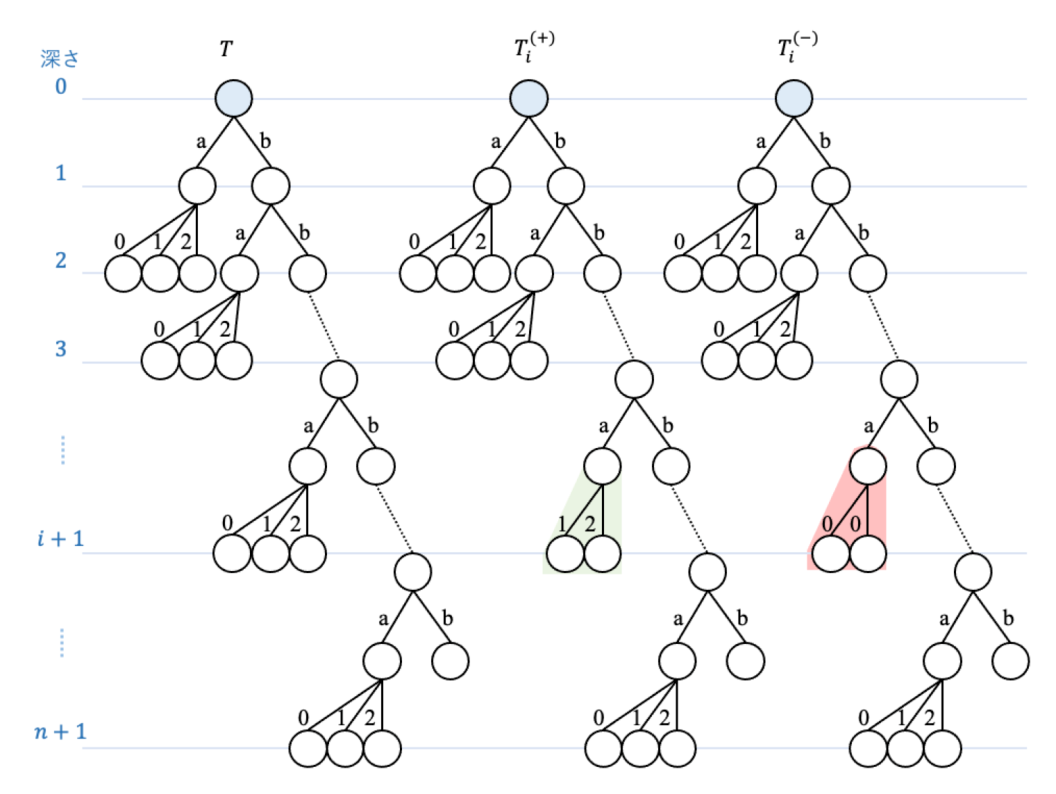
\includegraphics[scale=0.5]{sample-tree.eps}
  \caption{正例と負例の元となる無順序木$T$と正例の無順序木$T_{i}^{(+)}$,負例の無順序木$T_{i}^{(-)}$ $(1\leq i\leq n)$}\label{fig:sample-tree}
\end{figure}

% 図3.2
\begin{figure}[tb]
  \centering
  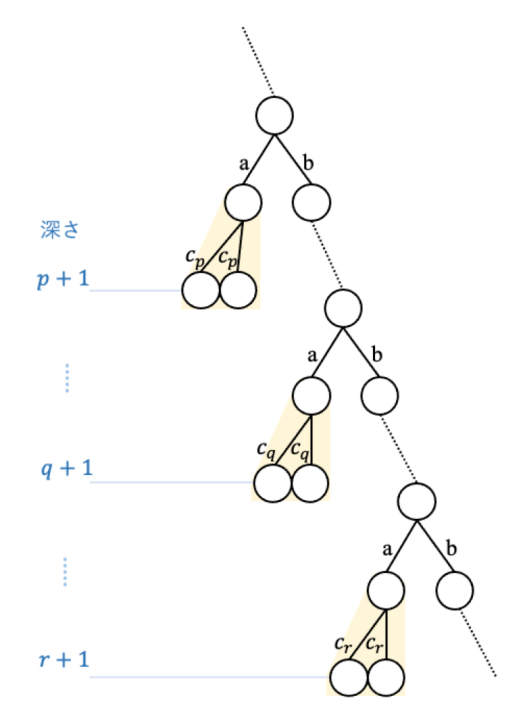
\includegraphics[scale=0.5]{clause-tree.eps}
  \caption{論理変数$x_p,x_q,x_r$ $(1\leq p < q < r \leq n)$のリテラルを含む節$C_k$ $(1\leq k\leq m)$に対する$T$ (図\ref{fig:sample-tree})の変更箇所}\label{fig:clause-tree}
\end{figure}

% 図3.3
\begin{figure*}[tb]
  \centering
  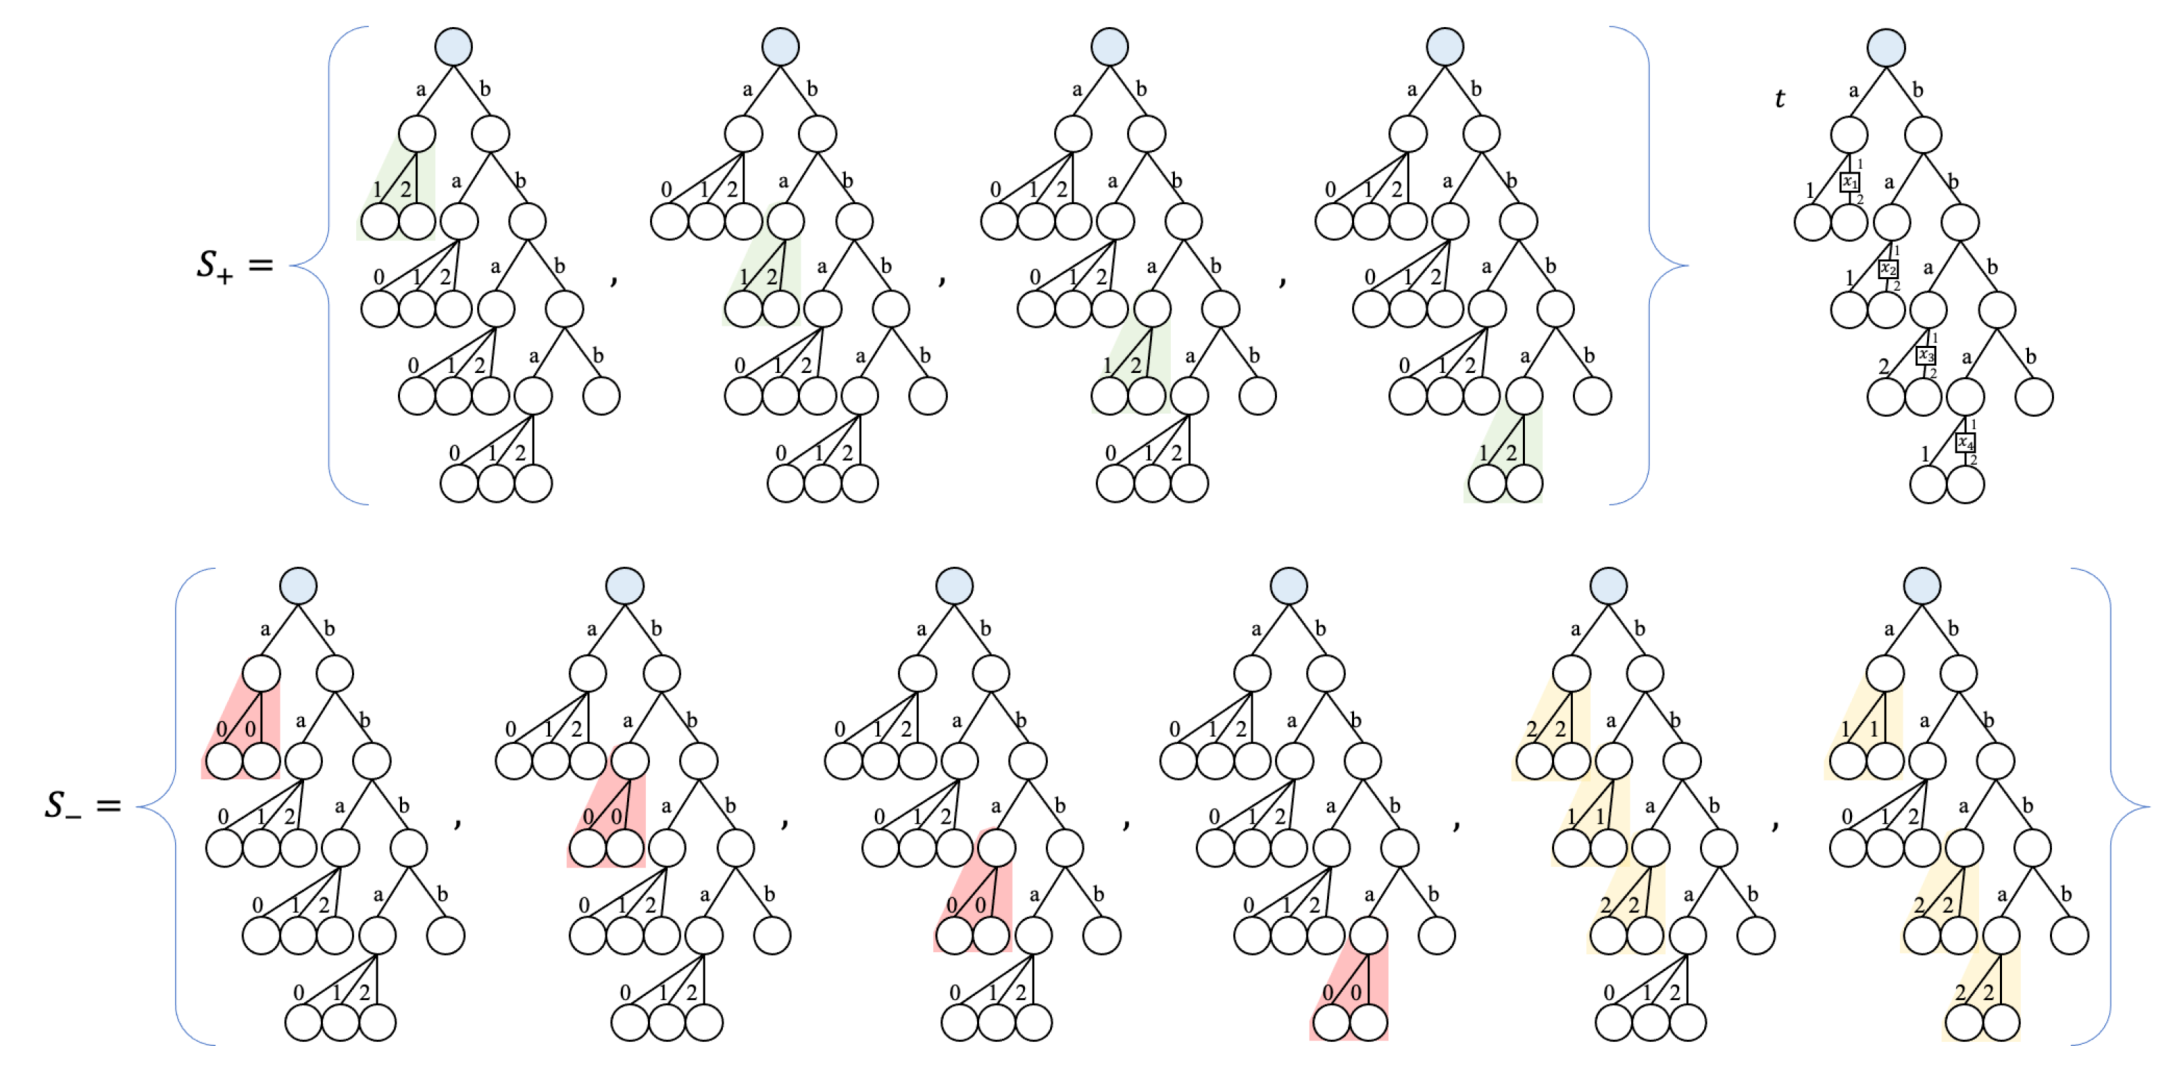
\includegraphics[scale=0.42]{example_npc.eps}
  \caption{多項式時間帰着の例: 3-CNF$F=(x_{1}\vee \bar{x_{2}}\vee x_{3})\wedge(\bar{x_{1}}\vee x_{3}\vee x_{4})$に対する$S_{+}$と$S_{-}$及び,$S_+\subseteq L(t)$かつ$S_-\cap L(t)=\emptyset$を満たす線形無順序木パターン$t\in {\cal LUTP}_{\Sigma,\Lambda,X}$}\label{fig:example_npc}
\end{figure*}

\noindent
\textbf{主張 1.}
3-CNF $F$から$S_{+}, S_{-}$への変換は多項式時間で計算可能である.
\smallskip

\noindent
(主張1の証明)
$F$に現れる論理変数$x_{1},\ldots,x_{n}$から,$T_{1}^{(+)},\ldots,T_{n}^{(+)}$及び$T_{1}^{(-)},\ldots,T_{n}^{(-)}$を得るには,論理変数$x_{i}$に対して,$T$の深さ$i+1$の葉の位置を求めるだけなので,全ての論理変数に対して$n\times O(n) = O(n^{2})$時間で計算することができる.次に,$F$に現れる節$C_k$ $(1\leq k\leq m)$に対して,その節$C_k$が論理変数$x_p,x_q,x_r$ $(1\leq p < q < r \leq n)$のリテラルを含むとき,$T$の深さ$p+1, q+1, r+1$の葉の位置を求めるだけなので,全ての節に対して$m\times O(n) = O(mn)$時間で計算することができる.以上より,この変換は$n$と$m$に関する多項式時間で計算することができる.
(主張1の証明終わり)

\medskip

\noindent
\textbf{主張 2.}
3-CNF $F$を充足可能とする論理変数への論理値割り当てが存在するならば,線形無順序木パターン$t$で$S_{+}\subseteq L(t)$かつ$S_{-}\cap L(t)=\emptyset$となるものが存在する.
\smallskip

\noindent
(主張2の証明)
$F$を充足可能とする論理変数の論理値割り当てにおいて,$x_{i}$ ($1\leq i\leq n$)の論理値が$true$のとき,$T$の深さ$i+1$ ($1\leq i\leq n$)の同じ親を持つ葉の親への辺で辺ラベル$0$の辺を変数とし,$2$を辺ラベルとする親へ辺を持つ葉を削除する.また,$x_{i}$ ($1\leq i\leq n$)の論理値が$false$のとき,$T$の深さ$i+1$ ($1\leq i\leq n$)の同じ親を持つ葉の親への辺で辺ラベル$0$の辺を変数とし,$1$を辺ラベルとする親へ辺を持つ葉を削除する.このようにして,$T$から線形無順序木パターン$t$を構成する.こうして構成した線形無順序木パターンは,$S_{+}$と$S_{-}$の構成方法から,$S_{+}\subseteq L(t)$かつ$S_{-}\cap L(t)=\emptyset$を満たす.
(主張2の証明終わり)

\medskip

\noindent
\textbf{主張 3.}
線形無順序木パターン$t$で$S_{+}\subseteq L(t)$かつ$S_{-}\cap L(t)=\emptyset$となるものが存在すれば,3-CNF $F$を充足可能とする論理変数への論理値割り当てが存在する.
\smallskip

\noindent
(主張3の証明)
線形無順序木パターン$t$が$S_{+}\subseteq L(t)$かつ$S_{-}\cap L(t)=\emptyset$を満たすとする.
$t$の高さ,すなわち葉の深さの最大値は$n+1$でなければならない.なぜなら,$T_{n}^{(+)}\in L(t)$かつ$T_{n}^{(-)}\not\in L(t)$が満たされており,それら2つの無順序木の違いは同じ親を持つ深さ$n+1$の葉の親への辺ラベルだけだからである.
$t$の各頂点の子の数は高々$2$である.
$t$の根は$2$つの子を持つ.
一方の辺ラベルは$a$であり,他方は$b$である.
$a$の辺ラベルを持つ辺で繋がった根からの頂点は高々$2$つの子を持つ.
そのうち1つは,同じ深さで$3$つの子を持つ$T_{2}^{(+)},\ldots,T_{n}^{(+)}$が全て$L(t)$に属することから,変数で繋がった子となる.
一方,もう1つのこは$T_{1}^{(-)}\not\in L(t)$であることから,辺ラベル$1$または$2$を持つ辺で繋がった子である.
同様の議論により,深さ$i+1$ ($2\leq i\leq n$)の同じ親を持つ葉は2つであり,1つは$1$または$2$を辺ラベルとして持つ辺で親と繋がり,他方は変数で親と繋がる.
ここで,深さ$n-1$の葉でない頂点は2つあるが,そのうち1つは辺ラベル$b$を持つ辺で葉と繋がるか,または変数で葉と繋がるかのいずれかである.
この線形無順序木パターン$t$から,次のようにして論理変数$x_{1},\ldots,x_{n}$への論理値割り当てを構成する.
深さ$i+1$ ($1\leq i\leq n$)の同じ親を持つ2つの葉に繋がる変数でない葉の親への辺ラベルが$1$のときは,$x_{i}$の論理値を$true$に,辺ラベルが$2$のときは,$x_{i}$の論理値を$false$にする.この論理値割り当ては,各節$C_{k}$ ($1\leq k\leq m$)に対する無順序木$T_{n+k}^{(-)}$が$L(t)$に含まれないことから,$C_{k}$に現れるリテラルが全て$false$になることはない.
したがって,$S_{+}\subseteq L(t)$かつ$S_{-}\cap L(t)=\emptyset$となる線形無順序木パターン$t$が存在すれば,3-CNF $F$を充足する論理変数の論理値割り当てが存在する.
(主張3の証明終わり)

\medskip

\noindent
主張1,2,3より,${\cal LUTP}$-${\cal CP}$はNP完全である.
\end{proof}

%\end{document}

% O(N^2)
% 3.3
\subsection{$O(N^2)$回の所属性質問による質問学習アルゴリズム}
線形無順序木パターン$t_*\in {\cal LUTP}_{\Sigma,\Lambda,X}$の所属性質問に答えるオラクルを${\cal O}(t_*)$と書く.アルゴリズム${\cal LUTP}$-${\cal QUERY}_{{\cal O}(t_{\ast})}^{Square}$ (アルゴリズム\ref{alg:lutp-query-square})は,Amoth\cite{amoth-ml2001}により提案されたアルゴリズムを応用したものである.ただし,Amothのアルゴリズムは,頂点を変数とみなす無順序木構造パターンに対するアルゴリズムであるので,辺を変数とみなす本論文の線形無順序木パターンでは,もし$|\Sigma|\not=\infty$かつ$|\Lambda|\not=\infty$ならば,そのままでは正しく動作しない.

$t_*$にマッチする無順序木$T$を入力とする.このとき,${\cal LUTP}$-${\cal QUERY}_{{\cal O}(t_{\ast})}^{Square}$は,もし$|\Sigma|=\infty$または$|\Lambda|=\infty$ならば,線形無順序木パターン$t\in {\cal LUTP}_{\Sigma,\Lambda,X}$で$L(t_*)=L(t)$となる$t$を,${\cal O}(t_*)$に対して$O(N^2)$回の所属性質問を行なって正しく出力することができる.ただし,$N$は$T$の頂点数である.そのときアルゴリズム{\sc Make\_Min\_Pos\_Tree\_Sqr} (アルゴリズム\ref{alg:lutp-query-square-step1})は$t_*$にマッチする$T$を入力とした場合,その出力として,$t_*$と同じ頂点数を持ち,かつ頂点数が最小となる正例を返す.まず$T$のうち,根から最も深い頂点とその頂点に接続する辺を削除し,これを$T'$とする.次に,オラクル${\cal O}(t_*)$に$T'$を問い合わせ,${\cal O}(t_*)(T')=Yes$であれば,$T$を$T'$で更新し,${\cal O}(t_*)(T')=No$であれば,削除した頂点と辺を元に戻す.さらに,処理がいくつか進んだ後に頂点や辺の削除が成功した場合,最も深い頂点から再び順に処理を行う.この操作を再帰的に繰り返し,$T$が変化しなくなると処理を終了する.この処理により,入力された$T$が$t_*$の構造を崩すことなく正確に反映しながら特定していく.その後,頂点数最小となった無順序木$T'$を入力とするとき,もし$|\Sigma|=\infty$または$|\Lambda|=\infty$ならば,アルゴリズム\ref{alg:lutp-query-square-step2} {\sc Variable\_Specify\_Sqr}は$t_*$と同型な$t$を出力する.

具体的には,正例の子の数を$c$とするとき,$T$に現れない頂点ラベルまたは辺ラベルを貼り付けた$c+1$個の辺と頂点(熊手型)を葉に接続し,${\cal O}(t_*)(T')=Yes$であればその葉を端点とする辺を変数に置き換え,${\cal O}(t_*)(T')=No$であれば変数に置き換えず,辺のままとする.このように熊手型を代入することにより変数か否かを決定する.しかし,もし$|\Sigma|\not=\infty$かつ$|\Lambda|\not=\infty$ならば,後述する図\ref{fig:counter_leaf_to_rake}のように変数を同定できないことがある.

% アルゴリズム1
\begin{algorithm}[tb]
\caption{{\sc Make\_Min\_Pos\_Tree\_Sqr};} \label{alg:lutp-query-square-step1}
\begin{algorithmic}[1]
  \Require{$t_{\ast}\in {\cal LUTP}$の正例$T\in L(t_{\ast})$, $t_{\ast}\in {\cal LUTP}$に対する所属性質問に答えるオラクル${\cal O}(t_{\ast})$;}
  \Ensure{$T\in L(t_{\ast})$;}
  \Function{Make\_Min\_Pos\_Tree\_Sqr}{$T$};
    \State $L\coloneqq T$の葉の集合;
    \While{$L\not= \emptyset$}
      \State $T'\coloneqq T$;
      \State $\ell$を$L$の葉の1つとする;
      \State $V'$から$\ell$,$E'$から$(p(\ell),\ell)$を削除,ただし$V'$と$E'$は$T'$の頂点集合と辺集合である;
      \If{${\cal O}(t_{\ast})(T')="Yes"$}
        \State $T\coloneqq T'$;
        \State $L\coloneqq T$の葉の集合;
      \Else
        \State $L$から$\ell$を削除;
      \EndIf
    \EndWhile
    \State \Return $T$;
  \EndFunction
\end{algorithmic}
\end{algorithm}

% アルゴリズム2
\begin{algorithm}[tb]
\caption{{\sc Variable\_Specify\_Sqr};} \label{alg:lutp-query-square-step2}
\begin{algorithmic}[1]
  \Require{最小正例$T\in L(t_{\ast})$, $t_{\ast}\in {\cal LUTP}$に対する所属性質問に答えるオラクル${\cal O}(t_{\ast})$;}
  \Ensure{$t\in {\cal LUTP}$;}
  \Function{Variable\_Specify\_Sqr}{$T$}
    \State $L\coloneqq T$の葉の集合; \,$c\coloneqq \max(\deg(T))$;
    \State$t\coloneqq T$;
    \For{$\ell\in L$}
      \State $T'\coloneqq T$の$\ell$に$c+1$個の子を接続;
      \If{${\cal O}(t_{\ast})(T')="Yes"$}
        \State $T\coloneqq T'$;
        \State $T'$の$(p(\ell),\ell)$に対応する$t$の辺ラベルを変数ラベルに更新;
      \EndIf
    \EndFor
    \State \Return $t$;
  \EndFunction
\end{algorithmic}
\end{algorithm}

% アルゴリズム3
\begin{algorithm}[tb]
\caption{${\cal LUTP}$-${\cal QUERY}_{{\cal O}(t_{\ast})}^{Square}$} \label{alg:lutp-query-square}
\begin{algorithmic}[1]
  \Require{$t_{\ast}\in {\cal LUTP}$の正例$T\in L(t_{\ast})$, $t_{\ast}\in {\cal LUTP}$に対する所属性質問に答えるオラクル${\cal O}(t_{\ast})$;}
  \Ensure{$t\in {\cal LUTP}$;}
  \State $T\coloneqq $ \Call{Make\_Min\_Tree\_Sqr}{$T$};
  \State $t\coloneqq $ \Call{Variable\_Specify\_Sqr}{$T$};
\end{algorithmic}
\end{algorithm}

% O(N)
% 3.4
\subsection{$O(N)$回の所属性質問による質問学習アルゴリズム}
本章では,1つの正例を入力とするアルゴリズム${\cal LUTP}$-${\cal QUERY}_{{\cal O}(t_{\ast})}^{Linear}$が正例のサイズの線形回数の所属性質問を用いて目標とする線形無順序木パターンを同定できることを示す.一般に次のように記号を定める.無順序木$T$と無順序木パターン$t$に対して,$\Theta_t(T)= \{\theta \mid t\theta\equiv T\}$とする.また,$T$と$t$の深さ$d$の葉の集合をそれぞれ$V_d(T)$と$V_d(t)$とする.$T$の高さを$h_T$とする.

学習対象である無順序木パターンを$t_{\ast}$とし, 無順序木$T\in L(t_{\ast})$を最初に与えられる正例とする.$\Theta_{t_{\ast}}(T)\neq\emptyset$である.$T$の葉を$v$とする.$v$から根に至る道を$P_v$とするとき,$P_v$上の頂点で,子の数2以上の頂点の最大深さを$\delta_v$とする.$P$上に子の数2以上の頂点がなければ$\delta_v=0$と定める.$t_{\ast}$の変数集合を$X(t_{\ast})$とする.$x\in X(t_{\ast})$に対して,$x$の子頂点の深さを$d_x$で表す.$X_j(t_{\ast})=\{x\in X(t_{\ast}\mid j=d_x)\}$とする.$t_{\ast}$への代入$\theta=\{x\coloneqq [T_x,\sigma_x]\mid x\in X(t_{\ast})\}$が$t_{\ast}\theta \equiv T$となるとき,$\theta$によって$x$に束縛される$T$の部分木$T_x$の葉$x$と$\sigma_v$のペアの全体を$\lambda_{\theta}(x)=\{v\mid v$は$\theta$における$T_x$の葉$\}$とし,$\lambda_{(\theta,k)}(x)=\{v\mid v\in \lambda_{\theta}(x)\land \lambda_v=k\}$とする.

% アルゴリズム4
\begin{algorithm}[tb]
\caption{{\sc Variable\_Number\_Specify\_Ln};} \label{alg:lutp-query-linear-step1}
\begin{algorithmic}[1]
  \Require{$t_{\ast}\in {\cal LUTP}$の正例$T\in L(t_{\ast})$, $t_{\ast}\in {\cal LUTP}$に対する所属性質問に答えるオラクル${\cal O}(t_{\ast})$;}
  \Ensure{$T\in L(t_{\ast})$;}
  \Function{Variable\_Number\_Specify\_Ln}{$T$}
    \State $h\coloneqq T$の高さ;
    \For{$d\in [1,2,\ldots,h]~(h\geq 1)$}
      \State $L_d\coloneqq T$の深さ$d$の葉の集合;
    \EndFor
    \For{$d\in [h,h-1,\ldots,1]~(h\geq 1)$}
      \For{$\ell_d\in L_d$}
        \State $T'\coloneqq T$の$\ell_d$に$P_{h-d+1}$となるように接続;
        \If{${\cal O}(t_{\ast})(T')="Yes"$}
          \State $T\coloneqq T'$;
        \EndIf
      \EndFor
      \For{$v\in L_{d-1}$}
        \State $C := \{c_i\mid T[c_i]\equiv P_{h-d+2}(1\leq i\leq n)\}$,ただし$c_1,\ldots,c_n(n\geq 2)$は$v$の子;
        \For{$c\in C$}
          \If{$|C|>1$}
            \State $C$から$c$を削除; % $c$ \textit{from} $C$
            \State $T$から$T[c],c,(p(c),c)$を削除;
            \If{${\cal O}(t_{\ast})(T')="Yes"$}
              \State $T\coloneqq T'$;
            \EndIf
          \EndIf
        \EndFor
      \EndFor
    \EndFor
    \State \Return $T$;
  \EndFunction
  %\State 長さ$k$のチェーン(長さ$k$の道だけからなる木,$k\geq 1$)に対して,次数1の頂点を根と定めた無順序木を$P_k$で表す.
  %\State 頂点$v$の親頂点を$p(v)$で表す
  %\State $T$の頂点$v$を根とする$T$の部分無順序木を$T[v]$と記述する
  %\State $h \gets \max(depth(T))$
\end{algorithmic}
\end{algorithm}

% 補題1
\begin{lemma}\label{lemma3.1}
  アルゴリズム{\sc Variable\_Number\_Specify\_Ln} (アルゴリズム\ref{alg:lutp-query-linear-step1})の入力を$T\in L(t_{\ast})$とする.このとき関数\Call{Variable\_Number\_Specify\_Ln}{$T$}は深さ$h+1$の葉の数が$t_{\ast}$の変数の数と等しい$t_{\ast}$の正例を出力する.
  深さ$d$に対する分岐を最小にする処理終了後の$T$を$T_d$とする.任意の$\theta\in\Theta_{(t_{\ast})}(T_d)$に現れる変数$x\in X_j(t_{\ast})$に対して,$j<d$のとき,任意の$k\geq d$に対して$\abs{\lambda_{(\theta,k)}(x)}=0$,$j\geq d$のとき,$\abs{\lambda_{\theta}(x)}=1$である.
\end{lemma}

% 証明
\begin{proof}
  深さ$d$に対する高さを揃える処理終了直後の正例を$T'_d$,分岐を最小にする処理終了直後の正例を$T_d$とする.$t_{\ast}$の高さは$h_T$以下であるので,もし$t_{\ast}$の正例に深さ$h_T+1$の頂点があれば,それは$t_{\ast}$の変数に束縛される無順序木の頂点である.\\

  $d=h_T$のとき:
  \begin{enumerate}
  \item[1] $\exists\theta\in \Theta_{t_{\ast}} (T)\forall v\in V_{h_T}(T)[\tilde{v}\in V_{h_T+1}(T_{h_T})\Leftrightarrow\exists x\in X(t_{\ast})[v\in\Delta_\theta(x)]],$
  \item[2] $\forall\theta\in\Theta_{t_{\ast}}(T_{h_T})\forall\tilde{v}\in V_{h_T+1}(T_{h_T})[\exists x\in X(t_{\ast})[\Delta_\theta(x)=\{\tilde{v}\}]\lor\forall x\in X(t_{\ast})[\tilde{v}\notin\Delta_{\theta,h_t-1}(x)]]$
  \end{enumerate}
  が成り立つ.これより,$d=h_T$のとき主張が示される.\\

  $1\leq d\leq h_T$のとき:
  \begin{enumerate}
    \item[1] $\exists\theta\in\Theta_{t_{\ast}}(T_{d+1})\forall v\in \bigcup_{k=d}^{h_T}V_k(T_{d+1})[\tilde{v}\in V_{h_T+1}(T_d)\Leftrightarrow\exists x\in X(t_{\ast})[v\in\Delta_\theta(x)]]$
  \end{enumerate}
  が成り立つ.なぜなら,$t_{\ast}$において深さ$d$の葉$u$が変数の子でないとき,任意の$\theta\in\Theta_{t_{\ast}}(T_d)$に対して,$T_d$の$u$に対応する頂点$v$は$T_d$の変数に束縛される葉ではない.したがって,$\tilde{v}\notin V_{h_t+1}(T_d)$である.
  
  深さ$d-1$以上において主張が正しいと仮定する.
  \begin{enumerate}
    \item[2] $\forall\theta\in\Theta_{t_{\ast}}(T_d)\forall\tilde{v}\in V_{h_T+1}(T_d)[\exists x \in X(t_{\ast})[\Delta_\theta(x)=\{\tilde{v}\}]\lor\forall x \in X(t_{\ast})\forall j\geq d-1[\tilde{v}\notin\Delta_{\theta,j}(x)]]$
  \end{enumerate}
  深さ$d$において,次の式が成り立つ.したがって,帰納的に主張が示される.
\end{proof}


% アルゴリズム5
\begin{algorithm}[tb]
\caption{{\sc Make\_Min\_Pos\_Tree\_Ln};} \label{alg:lutp-query-linear-step2}
\begin{algorithmic}[1]
  \Require{分岐数最小正例$T\in L(t_{\ast})$, $t_{\ast}\in {\cal LUTP}$に対する所属性質問に答えるオラクル${\cal O}(t_{\ast})$;}
  \Ensure{$T\in L(t_{\ast})$;}
  \Function{Make\_Min\_Pos\_Tree\_Ln}{$T$}
    \For{$d\in [1,2,\ldots,h]~(h\geq 1)$}
      \State $V_d\coloneqq L$の深さ$d$の部分集合;
      \For{$v\in V_d$}
        \If{$T[v]\equiv P_{h-d+1}$}
          \State $T$から$T[v]$を削除,ただし,$v$と$(p(v),v)$は削除しない;
          \If{$d\neq \max(depth(T))-1$}
            \If{${\cal O}(t_{\ast})(T')="Yes"$}
              \State $T\coloneqq T'$;
            \EndIf
          \Else
            \State $T\coloneqq T'$;
          \EndIf
        \EndIf
      \EndFor
    \EndFor
    \State \Return $T$;
  \EndFunction
\end{algorithmic}
\end{algorithm}


% 補題2
\begin{lemma}\label{lemma3.2}
  関数\Call{Variable\_Number\_Specify\_Ln}{$T$}の出力を$T\in L(t_{\ast})$とする.このときアルゴリズム\ref{alg:lutp-query-linear-step2} \Call{Make\_Min\_Pos\_Tree\_Ln}{$T$}は$t_{\ast}$の変数を辺に置き換えて得られる$t_{\ast}$の最小正例を出力する.
  深さ$d$に対する関数\Call{Make\_Min\_Pos\_Tree\_Ln}{$T$}終了後の$T$を$T_d$とする.任意の$\theta\in\Theta_{t_{\ast}}(T_d)$に対して,$\theta$に現れる変数$x\in X_j(t_{\ast})(1\geq j\geq d)$に束縛される無順序木はただ1つの辺から成る.
\end{lemma}


% 証明
\begin{proof}
  関数\Call{Variable\_Number\_Specify\_Ln}{$T$}終了後の$T$を$T_0$とする.任意の$\theta\in\Theta_{t_{\ast}}(T_{d-1})(d\geq1)$に対して,変数$x\in X_d(t_{\ast})$には,$P_{h_T-d+2}$が束縛されている.深さ$d$の処理後,$\abs{V_d(T_d)}=\abs{V_d(t_{\ast})}$となる.
  したがって,主張が示される.
\end{proof}


% アルゴリズム6
\begin{algorithm}[tb]
\caption{{\sc Variable\_Specify\_Ln};} \label{alg:lutp-query-linear-step3}
\begin{algorithmic}[1]
  \Require{最小正例$T\in L(t_{\ast})$, $t_{\ast}\in {\cal LUTP}$に対する所属性質問に答えるオラクル${\cal O}(t_{\ast})$;}
  \Ensure{$t\in {\cal LUTP}$;}
  \Function{Variable\_Specify\_Ln}{$T$}
    \State $h\coloneqq \max(depth(T))$
    \State $T=(V,E)$を左深さ優先木に更新;
    \For{$v\in V$}
      \State $c_1,\ldots,c_n(c\geq 2)\coloneqq v$の子,ただし,$T[c_1],T[c_2],\ldots,T[c_n]$は降順である;
      \For{$c\in [c_1,c_2,\ldots,c_n]$}
        \If{$T[c]$が長さ0以上のチェーン}
          \State $l\coloneqq T[c]$の葉;
          \State $T'\coloneqq T[c]$に$P_{h-d+1}$となるように接続;
          \If{${\cal O}(t_{\ast})(T')="Yes"$}
            \State $T\coloneqq T'$;
            \State $(p(v),v)$を変数$[p(v),v]$に更新;
          \EndIf
        \EndIf
      \EndFor
    \EndFor
    \State \Return $t$;
  \EndFunction
\end{algorithmic}
\end{algorithm}


関数\Call{Make\_Min\_Pos\_Tree\_Ln}{$T$}の出力$T$の頂点を左深さ優先順に処理する.以下では任意の$ v\in V(T)$の子$c_1,c_2,\ldots,c_m(m\geq2)$を根とする部分木$T[c_1],T[c_2],\ldots,T[c_m]$は左深さ優先順であるとする.頂点$v\in V(T)$の深さを$d_v$で表す.\par
$T$の子の数2以上の子孫を持つ頂点を左深さ優先順に帰りがけ順で並べた頂点列を$v_1,\ldots,v_{n'}(n'\geq1)$とする.$v_1,\ldots,v_{n'}$は処理が実行される頂点で,この頂点順に処理が終了する.すなわち,$v_{n'}$は$T$の根である.(本論文では,頂点$v$は$v$自身の子孫であるとする.)
また,アルゴリズム\ref{alg:lutp-query-linear-step3} {\sc Variable\_Specify\_Ln}内において,深さ$d_{v_i}$にある頂点$v_i$を根とする部分木$T[v_i]$の変数を特定する処理をFind\_Variable($T[v_i],d_{v_i}$)と記す.


% 補題3
\begin{lemma}\label{lemma3.3}
  関数\Call{Make\_Min\_Pos\_Tree\_Ln}{$T$}の出力を$T\in L(t_{\ast})$とする.このとき関数\Call{Variable\_Specify\_Ln}{$T$}は$t_{\ast}$を出力する.
  任意の$k(1\leq k\leq n')$に対して,$i(1\leq i\leq k)$に対するFind\_Variable($T[v_i],d_{v_i}$)が$t_{\ast}$の変数に対応する$T[v_i]$の辺を正しく特定しているとき,Find\_Variable($T[v_k],d_{v_k}$)は$t_{\ast}$の変数に対応する$T[v_k]$の辺を正しく特定する.
\end{lemma}


% 証明
\begin{proof}
  $v_{k-1},v_k(1<k\leq n')$の関係について場合分けにより証明する.
  \begin{enumerate}
    \item[(i)] $v_1$について:\\
                $T[v_1]$は左深さ優先順である.変数位置の特定には深さが$h_T+1$になるよう道を付加するので,$T[v_1]$が左深さ優先で最左であることが常に保証される.故にFind\_Variable($T[v_1],d_{v_1}$)は$t_{\ast}$の変数に対応する$T[v_1]$の辺を正しく特定する.
    \item[(ii)] $v_k$が$v_{k-1}$の親であるとき:\\
                $v_k$の子に対するFind\_Variableは全て正しく終了している.よって,$t_{\ast}$の変数に対応する$T[v_k]$の辺は既に正しく特定されている.
    \item[(iii)] $v_k$が$v_{k-1}$の兄弟であるとき:\\
                $v$を$v_k$の任意の真の先祖,$v$の子を$c_1,\ldots,c_m(m\geq2)$とし,$T[c_j](1\leq j\leq m)$が$v_k$を含むとする.$c_1,\ldots,c_m$に対応する$t_{\ast}$の頂点を$c'_1,\ldots,c'_m(m\geq2)$とする.Find\_Variable($T[c_j],d_{c_j}$)が実行されているとき,任意の$\beta(j<\beta\leq m)$に対して,$T[c_\beta]$が$T[c_j]$と異なる深さ列を持つならば,$t_{\ast}[c'_j]$が$T[c_\beta]$にマッチすることはない.\\
                なぜなら,無順序木パターンがその深さ列より小さい無順序木にマッチすることはないからである.$T_[c_\beta]$が$T[c_j]$と同じ深さ列を持つならば,$T[c_j]$の処理における$t_{\ast}[c'_j]$の変数位置は,$T[c_\beta]$に対応する$t_\ast [c'_j]$の変数位置より深さ優先で特定される.\\
                一方,任意の$\alpha(1\leq\alpha<j)$では,既にFind\_Variable($T[c_\alpha],d_{c_\alpha}$)の実行は終了しているので,$T[c_\alpha]$における$t_\ast [c'_\alpha]$に対応する変数の位置は特定されている.もし,Find\_Variable($T[c_j],d_{c_j}$)を実行中の$T[c_j]$に$\gamma '(\gamma '<j)$が存在して$t_\ast[c'_{\gamma '}]$がマッチすれば,$\gamma(\gamma<j)$が存在して$t_\ast [c'_j]$はすでに変数位置が特定されている$T[c_\gamma]$にマッチする.\\
                このとき$T[c_\gamma]$の深さ列は$T[c_j]$のそれ以上なので,Find\_Variable($T[c_j],d_{c_j}$)の実行中に変数判定を行う辺は,$T[c_\gamma]$において既に変数であると判定されている.したがってFind\_Variable($T[c_j],d_{c_j}$)は$T[c_j]$の変数位置を正確に特定する.
                以上より,Find\_Variable($T[c_j],d_{c_j}$)で実行されるFind\_Variable($T[v_k],d_{v_k}$)も$t_\ast$の変数に対応する$T[v_k]$の辺を正しく特定する.
    \item[(iv)] $v_k$が$v_{k-1}$の兄弟の子孫であるとき:\\
                $v_k$と$v_{k-1}$の共通の先祖$v$について(iii)と同様に示される.
  \end{enumerate}
\end{proof}

% アルゴリズム7
\begin{algorithm}[tb]
\caption{${\cal LUTP}$-${\cal QUERY}_{{\cal O}(t_{\ast})}^{Linear}$} \label{alg:lutp-query-linear}
\begin{algorithmic}[1]
  \Require{$t_{\ast}\in {\cal LUTP}$の正例$T\in L(t_{\ast})$, $t_{\ast}\in {\cal LUTP}$に対する所属性質問に答えるオラクル${\cal O}(t_{\ast})$;}
  \Ensure{$t\in {\cal LUTP}$;}
  \State $T\coloneqq $ \Call{Variable\_Number\_Specify\_Ln}{$T$};
  \State $T\coloneqq $ \Call{Make\_Min\_Tree\_Ln}{$T$};
  \State $t\coloneqq $ \Call{Variable\_Specify\_Ln}{$T$};
\end{algorithmic}
\end{algorithm}

% 定理2
\begin{theorem}\label{theorem3}
  無順序木パターン$t_{\ast}\in {\cal LUTP}_{\Sigma, \Lambda, X}$に対する所属性質問に答えるオラクル${\cal O}(t_{\ast})$を仮定する.
  頂点数$N(N\geq 5)$の正例$T\in L(t_{\ast})$が与えられたとき,${\cal O}(t_{\ast})$への高々$4N$回の所属性質問を行うことで,$t_\ast$の表現,すなわち$L(t_\ast)=L(t)$となる線形無順序木パターン$t\in{\cal LUTP}$を同定可能である.
  %(1)線形無順序木パターン$t_{\ast}\in{\cal LUTP}_{\Sigma,\Lambda,X}$に対する所属性質問に答えるオラクル${\cal O}(t_{\ast})$を仮定する.頂点数$N$の正例$T\in L(t_{\ast})$が与えられたとき,${\cal O}(t_{\ast})$への$O(N)$回の所属性質問を行うことで,$L(t_{\ast})=L(t)$となる無順序木パターン$t\in{\cal LUTP}_{\Sigma,\Lambda,X}$を同定可能である.
  %(2)無順序木パターン$t_{\ast}\in {\cal LUTP}_{\Sigma, \Lambda, X}$に対する所属性質問に答えるオラクル$\mathcal{O}(t_{\ast})$を仮定する.頂点数$N(N\geq 5)$の正例$T\in L(t_{\ast})$が与えられたとき,$\mathcal{O}(t_{\ast})$への高々$4N$回の所属性質問により,$t_{\ast}$の表現,すなわち$t=(V_t, E_t, H_t)$を同定可能である.
\end{theorem}

\begin{proof}
  正例の無順序木の頂点数を$N$とするとき,アルゴリズム\ref{alg:lutp-query-linear-step1}の6--12行において,深さごとにチェーン型の無順序木を代入して,オラクルに問い合わせを行う回数は高々$N$回,15--23行において,深さごとに分岐を削除して,オラクルに問い合わせを行う回数は高々$N$回である.アルゴリズム\ref{alg:lutp-query-linear-step2}において,根に近い道の長いチェーン型の無順序木を順に短くして,オラクルに問い合わせを行う回数は高々$N$回である.アルゴリズム\ref{alg:lutp-query-linear-step3}において,葉にチェーン型の無順序木を代入して,高々$N$回オラクルへの所属性質問で変数か否かを判定する.したがって,合計で${\cal O}(t_{\ast})$への高々$4N$回の所属性質問を行うことで,$t_\ast$の表現,すなわち$L(t_\ast)=L(t)$となる線形無順序木パターン$t\in{\cal LUTP}$を同定可能である.アルゴリズムの正当性は,補題\ref{lemma3.1}, \ref{lemma3.2}, \ref{lemma3.3}より証明される.以上より,本定理が得られる.
\end{proof}

% 3.5
\subsection{質問戦略に関する考察}
これより,アルゴリズム${\cal LUTP}$-${\cal QUERY}_{{\cal O}(t_{\ast})}^{Linear}$(アルゴリズム\ref{alg:lutp-query-linear})を設計するにあたり,発生した問題点と改善点を述べる.

まず,はじめのアプローチとして,最小正例の発見と変数の特定を同時に行うために正例集合に現れる子の頂点数$c$に1を加えた$c+1$個の葉を持つ構造を生成し,これを熊手型と呼ばれる無順序木として葉に代入する手法(以降,熊手戦略と呼ぶ)を採用した.具体的には,アルゴリズム${\cal LUTP}$-${\cal QUERY}_{{\cal O}(t_{\ast})}^{Square}$では関数\Call{Make\_Min\_Tree\_Sqr}{$T$}において辺を削除することで最小正例を発見し,関数\Call{Variable\_Specify\_Sqr}{$T$}において熊手戦略を用いることによって変数を特定していた.そこで,この2つのステップを同時に行うことで既存手法より質問回数の少ないアルゴリズムを開発し,目標の線形無順序木パターンを発見することを試みた.しかし,図\ref{fig:counter_leaf_to_rake}に示す例によりパターンを発見することが困難であることが確認できた.具体的には,葉に直接,熊手型を接続するため,無順序木の性質上,接続された熊手型の無順序木が,同様の構造を持つ他の部分木にも適用されてしまう可能性がある.その結果,線形無順序木パターンから見ると本来は代入すべきでない箇所にも誤って熊手型の無順序木が代入されてしまい,対象とする構造が正確に反映されない問題が生じる.このように,構造を横方向に広げて処理を進める熊手戦略は,無順序木のように見かけ上一意に定まらない構造に対しては不適切であることが確認できた.

熊手戦略では,無順序木の性質に起因する誤代入が生じやすく,正例の構造を正確に反映することが困難である.そこで,正例となる無順序木の高さを$H_T$とした場合,葉に対して$H_T$よりも1長い位置まで道を付加する方法を取る.この手法は,構造を縦方向に広げながら処理を進めることからチェーン戦略と呼ぶ.チェーン戦略の特徴は,縦方向に構造を拡張することで分岐を持たない無順序木を代入する点にある.このアプローチにより,無順序木の特性に依存した代入の曖昧性が解消され,他の部分木に誤って適用されることがない.結果として,正例の構造を正確に反映しながら,正確な処理が可能となる.チェーン戦略は,無順序木における構造の一意性を保証し,パターンの特定において重要な役割を果たす.

% 図3.4
\begin{figure*}[tb]
  \centering
  \includegraphics[scale=0.6]{fig/fig-counter_leaf_to_rake.eps}
  \caption{線形無順序木パターン$t$と正例となる無順序木$T$に対して,熊手戦略を用いて辺縮約と変数同定を同時に処理すると,本来であれば変数として扱うべきでない辺を誤って変数と位置づけてしまう問題が生じる.}\label{fig:counter_leaf_to_rake}
\end{figure*}

次に,チェーン型の無順序木を葉に代入し,高さを揃えることで目標とする線形無順序木パターンを発見できることが確認できた.一見すると関数\Call{Make\_Min\_Tree\_Sqr}{$T$}まででパターンを発見できているように見えるがそうではない.図\ref{fig:counter_step1_2}に具体例を示す.上段では,関数\Call{Variable\_Number\_Specify\_Ln}{$T$}の処理を示している.このアルゴリズムが終了した段階では,正例として与えられる無順序木の高さ$H_T$を超える位置に道を追加することで,変数の数と分岐の数が一致することを確認できる.この処理により,無順序木における変数の位置や数が適切に特定され,次の処理への準備が整う.
一方で,最小の正例を特定する関数\Call{Make\_Min\_Tree\_Ln}{$T$}(図\ref{fig:counter_step1_2}の下段)では,無順序木の持つ特性が障害となる場合がある.具体的には,削除を行う順番が影響を及ぼし,削除が完了した部分が定数として誤って解釈される可能性が生じる.このような場合,処理の進行中に本来変数とみなすべき箇所が定数とみなされることで,意図した通りの変数の位置を特定できなくなるリスクがある.そのため,最小の正例を発見する処理とは別で変数を特定する処理が必要である.

% 図3.5
\begin{figure*}[tb]
  \centering
  \includegraphics[scale=0.5]{fig/fig-counter_step1_2.eps}
  \caption{線形無順序木パターン$t$と正例となる無順序木$T$に対して,最小正例を発見するまでで処理を終了すると,熊手型の無順序木が存在する箇所と変数であるべき位置が一致しないため,パターンの発見には至らない.}\label{fig:counter_step1_2}
\end{figure*}

しかし,関数\Call{Make\_Min\_Tree\_Sqr}{$T$}終了後,無順序木を対象としているため,必ずしも見かけ上同型の最小正例を発見することができない.そこで,本研究では無順序木の構造を一意に定めるために左深さ優先木を導入した.左深さ優先木とは,無順序木における各頂点の子の順序を深さ列が最大となるように並び替えて構築される一意に定められる木構造である.この定義に基づき,まず無順序木を左深さ優先木に変換して,構造を一意化する.これにより,アルゴリズム処理における誤解釈の可能性を取り除くことで正確な処理が可能となる.さらに,左深さ優先木への変換によって得られる一意性は,変数の位置特定の処理において重要な役割を果たす.図\ref{fig:counter_ldfs_tree}では,左深さ優先木に変換した場合と変換しない場合の違いを具体的に示している.上段は,図\ref{fig:counter_step1_2}の続きから左深さ優先木に変換しない場合を示しており,この場合,変数を特定する順番が一意に定まらず,代入が正しく行われない場合がある.その結果,変数を正確に特定することができず,対象とする木構造を完全には反映できない.一方,下段では左深さ優先木に変換した場合の結果を示している.この場合,左深さ優先の基準に基づいて木構造を一意に定めている.その上で,チェーン戦略を用いることにより,変数を特定することが可能になる.具体的には,代入したチェーン型の無順序木の深さ列が左の部分木の深さ列を超えることがないため,変数の代入が正確に行われる.この手法により,元の無順序木パターンを忠実に再現することが可能になる.

% 図3.6
\begin{figure*}[tb]
  \centering
  \includegraphics[scale=0.5]{fig/fig-counter_ldfs_tree.eps}
  \caption{線形無順序木パターン$t$と正例となる無順序木$T$に対して,最小正例が得られた場合でも,無順序木である特性上,変数を特定する順番によっては元のパターンを再現できないことがある(図上).一方で,左深さ優先木に変換することで無順序木が一意に定まるため,元のパターンを正確に再現することが可能となる(図下).}\label{fig:counter_ldfs_tree}
\end{figure*}

% 3.6
\subsection{アルゴリズム${\cal LUTP}$-${\cal QUERY}_{{\cal O}(t_{\ast})}^{Linear}$の実験的解析}
人工データを用いて行なった2つの計算機実験による解析結果を報告する.本実験では${\cal LUTP}$の所属性質問を行う際のオラクルとして,Shoudaiら\cite{shoudai-ieice2018}によって提案された線形無順序項木パターンの多項式時間マッチングアルゴリズムを使用した.このアルゴリズムは,学習目標である無順序木パターン$t_\ast\in{\cal LUTP}$から照合のためのルールを作成して無順序木$T$の頂点と$t_\ast$の頂点の間の対応関係を求める.それにより$t_\ast$が$T$とマッチするか否かを判定する.

% 3.6.1
\subsubsection{最小正例から同定する際の質問回数の解析} \label{qltimes_input_min}
オラクル${\cal O}(t_\ast)$を用いた質問学習アルゴリズム${\cal LUTP}$-${\cal QUERY}_{{\cal O}(t_{\ast})}^{Linear}$の入力を$t_\ast$の変数を辺とみなした無順序木$T_{t_\ast}$として各ステップでオラクル${\cal O}(t_\ast)$に所属性質問を行う回数を求める.すなわち,アルゴリズム${\cal LUTP}$-${\cal QUERY}_{{\cal O}(t_{\ast})}^{Linear}$への入力を,学習目標である$t_\ast\in{\cal LUTP}$の頂点数最小の正例とする.ここでは,あらかじめ定められた頂点数を持つ全ての無順序木を解析対象とするために,無順序木の列挙アルゴリズム\cite{nii-nakano_uno2003,cs-nakano_uno2004}を使用して,頂点数21まで全無順序木を生成した.生成した各無順序木の葉辺を変数に置き換えることによって,全ての無順序木パターンを作成して,頂点数と所属性質問を行う回数に関する解析を行った.ただし,頂点数2から13は全ての無順序木パターンに対して解析を行なったが,頂点数14以降は計算時間が非常に大きくなるため,頂点数13の無順序木パターンの数409963個を参考に410000個の無順序木パターンをランダムに生成して解析を行った.

実験結果の折れ線グラフを図\ref{fig:qltimes_input_min}に,その数値結果を表\ref{tbl:qltimes_input_min}に示す.横軸に頂点数,縦軸に質問回数を表す.各頂点の質問回数に対して最大値を青色,最小値を緑色,平均値を橙色でプロットして折れ線グラフで表現する.いずれも定数倍で増加していることが確認できる.全ての無順序木パターンを解析した頂点数13までの結果から,頂点数を$N(N\geq5)$とするとき,質問回数の最大値が$4(N-2)$(図\ref{fig:qltimes_input_min}: 青破線),最小値が4(図\ref{fig:qltimes_input_min}: 緑破線)であることが確認できる.
実験により,質問回数が最大となる無順序木パターン$t_{max}$は,$N\geq5$の場合,葉辺が変数である長さ2のチェーンが1つと葉辺に変数を持つ長さ1のチェーンが2以上ある場合であることが確認できる(図\ref{fig:qltimes_max_min}(左)).これは根と$N-1$個の葉が接続された無順序木パターンに比べ,アルゴリズム\ref{alg:lutp-query-linear-step2}で深さ1または2のどちらが変数であるか検証する必要があるため質問回数が多くなる.$N=2,3,4$の場合の最大質問回数はそれぞれ3,6,9である.また,質問回数が最小となる無順序木パターン($N\geq3$)は図\ref{fig:qltimes_max_min}の右に示す無順序木パターン$t_{min}$である.図\ref{fig:qltimes_max_min}では$t_{min}$の頂点集合を$\{u_1,u_2,\ldots,u_n\}~(n=N,N\geq3)$としている.根$u_1$から頂点$u_{n-2}$まで分岐を持たない頂点が接続されており,$u_{n-2}$に接続する長さ1のチェーンで葉辺が変数であるものが1つ,葉辺が辺であるものが1つ持つ場合である.この無順序木パターンは,頂点数$N$のチェーンである無順序木パターンに比べ,アルゴリズム\ref{alg:lutp-query-linear-step2}でのチェーンを短くするための質問を行う必要がない.そのため,質問回数が最小となる.

% 図3.7, 表3.1
\begin{figure}[tb]
  \begin{center}
  % 図
 % \begin{minipage}[c]{0.5\hsize}
 %   \centering
    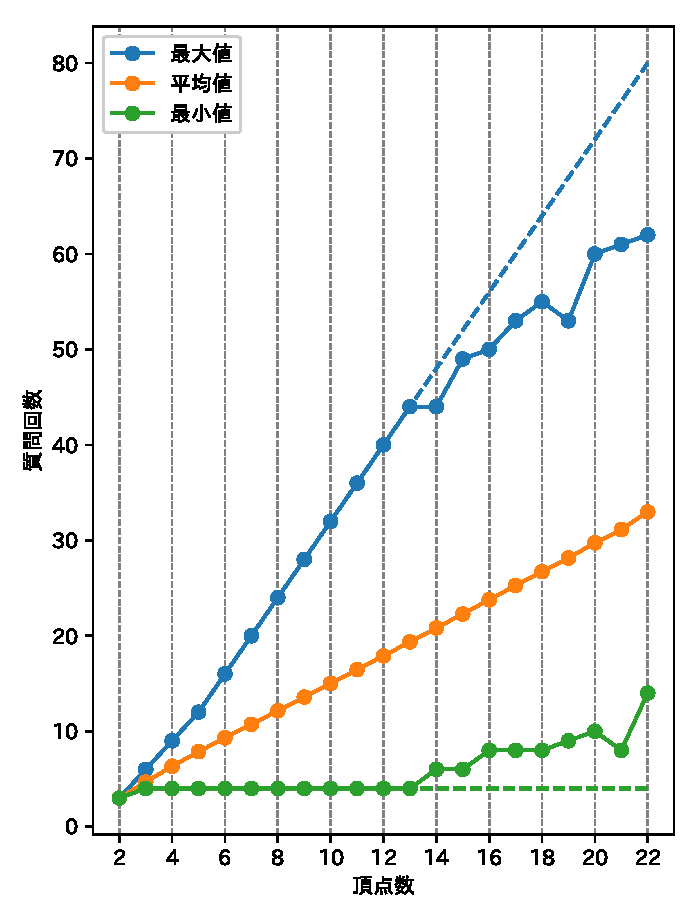
\includegraphics[scale=0.7]{fig/fig-qltimes_input_min.eps}
    \caption{入力が最小正例とするときの質問回数の推移}\label{fig:qltimes_input_min}
 % \end{minipage}
  %\hspace{0.02\hsize} % ここで隙間作成
  \vspace*{10.5pt}
  % 表
 % \begin{minipage}[c]{0.5\hsize} % 表を並べることが可能
 %   \centering
    \tblcaption{図\ref{fig:qltimes_input_min}の数値結果}\label{tbl:qltimes_input_min}
    \begin{tabular}{rrrrr} \hline
      頂点数 &  木の数 & 最大値 & 最小値 & 平均値 \\ \hline\hline
          2 &      1 &     3 &     3 &  3.00 \\
          3 &      3 &     6 &     4 &  4.67 \\
          4 &      9 &     9 &     4 &  6.33 \\
          5 &     28 &    12 &     4 &  7.86 \\
          6 &     88 &    16 &     4 &  9.31 \\
          7 &    284 &    20 &     4 & 10.73 \\
          8 &    927 &    24 &     4 & 12.15 \\
          9 &   3074 &    28 &     4 & 13.57 \\
         10 &  10300 &    32 &     4 & 15.01 \\
         11 &  34880 &    36 &     4 & 16.45 \\
         12 & 119109 &    40 &     4 & 17.90 \\
         13 & 409963 &    44 &     4 & 19.35 \\
         14 & 410000 &    44 &     6 & 20.82 \\
         15 & 410000 &    49 &     6 & 22.28 \\
         16 & 410000 &    50 &     8 & 23.77 \\
         17 & 410000 &    53 &     8 & 25.27 \\
         18 & 410000 &    55 &     8 & 26.72 \\
         19 & 410000 &    53 &     9 & 28.14 \\
         20 & 410000 &    60 &    10 & 29.73 \\
         21 & 410000 &    61 &     8 & 31.12 \\ \hline
    \end{tabular}
 % \end{minipage}
  \end{center}
\end{figure}
0
% 図3.8
\begin{figure}[tb]
  \centering
  \includegraphics[scale=0.34]{fig/fig-qltimes_max_min.eps}
  \caption{頂点数が同じとき質問回数が$4(N-2)$~($N$は入力となる正例の頂点数)で最大となる無順序木パターン$t_{max}$と,4で最小となる無順序木パターン$t_{min}$}\label{fig:qltimes_max_min}
\end{figure}

% 3.6.2
\subsubsection{正例の葉の数に関する質問回数の解析}
アルゴリズム${\cal LUTP}$-${\cal QUERY}_{{\cal O}(t_{\ast})}^{Linear}$への入力の頂点数を,学習目標である$t_\ast\in{\cal LUTP}$の頂点数の1倍から2倍まで変化させて,正例の葉の数に関する質問回数の解析を行なった.\ref{qltimes_input_min}項において全ての無順序木パターンを調査することができた頂点数13を対象とし,頂点数13から成る無順序木パターン$t_\ast$に対して,正例となる頂点数26の無順序木をランダムに100個生成した.生成した正例の集合を$S_+$とする.$S_+$に属す無順序木を${\cal LUTP}$-${\cal QUERY}_{{\cal O}(t_{\ast})}^{Linear}$の入力として,アルゴリズム\ref{alg:lutp-query-linear-step1}まで行う.これをランダムに40000回繰り返した.異なる入力(無順序木)であっても学習目標である無順序木パターン$t_\ast$が同じであれば,無順序木の頂点数に関わらずアルゴリズム\ref{alg:lutp-query-linear-step2}とアルゴリズム\ref{alg:lutp-query-linear-step3}の質問回数は変わらないので,本実験はアルゴリズム\ref{alg:lutp-query-linear-step1}まで実行する.その結果を下記に解析する.

実験結果の折れ線グラフを図\ref{fig:qltimes_input_twice}に,その数値結果を表\ref{tbl:qltimes_input_twice}に示す.入力となる無順序木の頂点数を固定した場合,質問回数は無順序木の葉の数に比例して増加することが確認できる.質問回数は,無順序木の頂点数に関わらず,葉の数のみに依存する.また,アルゴリズム\ref{alg:lutp-query-linear-step1}までの質問回数は葉の数の2倍以下であることが確認できる.これは,葉にチェーン型を代入するステップと分岐を減らすステップを同じ深さで行っているからである.すなわち,定理\ref{theorem3}と同じ結果になることが確認できる.

% 図3.9, 表3.2
\begin{figure}[tb]
  \begin{center}
  % 図
  %\begin{minipage}[c]{0.5\hsize}
  %  \centering
    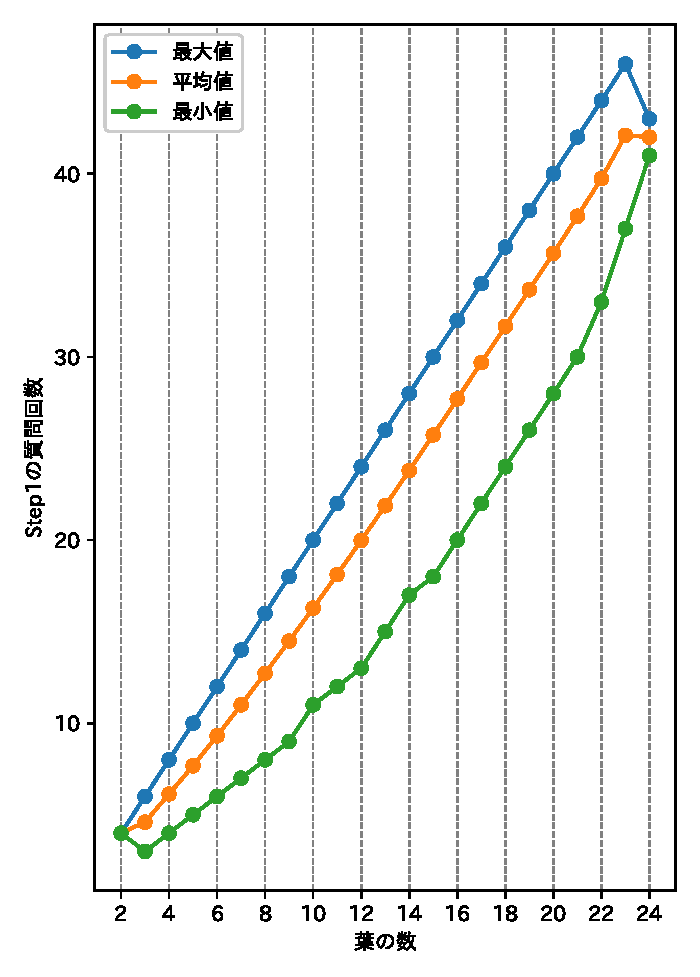
\includegraphics[scale=0.7]{fig/fig-qltimes_input_twice.eps}
    \caption{入力が最小正例とするときの質問回数の推移}\label{fig:qltimes_input_twice}
  %\end{minipage}
  %\hspace{0.02\hsize} % ここで隙間作成
  \vspace*{10.5pt}
  % 表
  %\begin{minipage}[c]{0.5\hsize} % 表を並べることが可能
  %  \centering
    \tblcaption{図\ref{fig:qltimes_input_twice}の数値結果}\label{tbl:qltimes_input_twice}
    \begin{tabular}{rrrrr} \hline
      葉の数 &   木の数 & 最大値 & 最小値  & 平均値 \\ \hline\hline
          2 &       1 &     4 &     4  &  4.00 \\
          3 &      15 &     6 &     3  &  4.60 \\
          4 &     238 &     8 &     4  &  6.13 \\
          5 &    3747 &    10 &     5  &  7.67 \\
          6 &   30859 &    12 &     6  &  9.31 \\
          7 &  168767 &    14 &     7  & 11.00 \\
          8 &  646945 &    16 &     8  & 12.73 \\
          9 & 1802648 &    18 &     9  & 14.49 \\
         10 & 3764760 &    20 &     11 & 16.29 \\
         11 & 6030044 &    22 &     12 & 18.12 \\
         12 & 7557200 &    24 &     13 & 19.98 \\
         13 & 7537840 &    26 &     15 & 21.88 \\
         14 & 6050538 &    28 &     17 & 23.80 \\
         15 & 3945616 &    30 &     18 & 25.74 \\
         16 & 2099413 &    32 &     20 & 27.71 \\
         17 &  914576 &    34 &     22 & 29.69 \\
         18 &  324500 &    36 &     24 & 31.67 \\
         19 &   92965 &    38 &     26 & 33.67 \\
         20 &   21257 &    40 &     28 & 35.66 \\
         21 &    3855 &    42 &     30 & 37.68 \\
         22 &     484 &    44 &     33 & 39.73 \\
         23 &      30 &    46 &     37 & 42.10 \\
         24 &       2 &    43 &     41 & 42.00 \\ \hline
    \end{tabular}
 % \end{minipage}
\end{center}
\end{figure}
